\documentclass[10.5pt]{article}
\usepackage[letterpaper,margin=0.9in]{geometry}
\usepackage[scaled]{helvet}
\renewcommand{\familydefault}{\sfdefault}
\renewcommand{\ttdefault}{cmtt}
\usepackage{amsmath}
\usepackage{booktabs,tabularx,array}
\usepackage{graphicx}
\usepackage[font=small,labelfont=bf]{caption}
\usepackage{enumitem}
\usepackage[hidelinks]{hyperref}
\usepackage{float}
\usepackage{titlesec}
\titleformat{\section}{\large\bfseries}{\thesection.}{0.5em}{}
\titleformat{\subsection}{\normalsize\bfseries}{\thesubsection}{0.5em}{}
\titlespacing*{\section}{0pt}{1.1em}{0.4em}
\setlist{nosep,leftmargin=1.3em}
\setlength{\parskip}{0.45em}
\setlength{\parindent}{0pt}
\renewcommand{\arraystretch}{1.15}

\begin{document}
{\LARGE\bfseries Midterm Results Pack}\\[0.3em]
{\large DSC 261 Group 3: position and format bias in Qwen3 judges}\\[0.2em]
{\small For the team writing the midterm report. Every number below comes from the raw judge logs, generated
by \url{scripts/report_stats.py} and \url{scripts/report_extra.py}. Last updated 9 Nov 2026.}

\section{Summary}
\begin{itemize}
\item \textbf{What ran.} 100 frozen Chatbot Arena pairs $\times$ 10 judge calls per pair $\times$ 8 judge setups
(Qwen3 0.6B, 1.7B, 4B and 8B, each with thinking off and on) gives \textbf{8{,}000 judge calls, with 0 invalid
answers}.
\item \textbf{Position bias is large.} Swapping the order of the two answers changes the verdict far more often
than chance, by 15--73.5 percentage points beyond noise, in 7 of 8 setups.
\item \textbf{Thinking reduces position bias but does not remove it.} The average drop is 30.5 points (18.3 points
excluding 0.6B). With thinking on, 1.7B, 4B and 8B still sit at 15--16.5 points.
\item \textbf{Format bias is small.} Removing markdown rarely changes which answer wins. But 4 of 8 setups pick
the version that kept its markdown 53.5--58\% of the time (significantly above the no-bias 50\%).
\item \textbf{Hypothesis H1} (for the largest judge with thinking, the lower end of the 95\% CI of the excess
flip rate is above 2 points): \textbf{yes for position} (8B with thinking: 15.0 points, CI 5.0--25.5).
\textbf{Not shown for format} on the pre-registered measure (format excess flip $-1.0$, CI $-6.2$ to 4.2).
Markdown preference, the more sensitive measure, is also not significant for this setup (52.0\%).
\item \textbf{Agreement with human voters is weak.} It is 51--66\%, close to a ``pick the longer answer'' rule (57\%).
\end{itemize}

\section{What we ran}
\begin{table}[H]
\centering\small
\begin{tabularx}{\linewidth}{>{\bfseries}p{3.0cm} X}
\toprule
Data & 100 pairs from Chatbot Arena: 84 from the 2025 release and 16 from 2023. Both answers in every pair use
markdown. All pairs are English, single-turn, with a clear human winner (no ties). Answer lengths are within 2$\times$
of each other, and no answer contains code or a table. \\
Judge prompt & The standard MT-Bench pairwise judge prompt, with the tie option removed. The judge must answer
[[A]] or [[B]]. \\
Calls per pair & 10 (Table~\ref{tab:design}): both orders; both orders repeated (to measure noise); and versions
with one or both answers' markdown removed. \\
Judges & Qwen3 at 0.6B and 1.7B (full precision), 4B (8-bit), 8B (4-bit AWQ). Each runs with thinking off and on. \\
Settings & Each mode uses the sampling settings from the model card. Thinking is capped at 2{,}048 tokens.
An unreadable answer is retried once (never needed). \\
Hardware & 0.6B--4B ran on a MacBook (M2 Pro, MLX). 8B ran on an RTX 3070 laptop GPU (vLLM). \\
\bottomrule
\end{tabularx}
\end{table}

\begin{table}[H]
\centering\small
\caption{The 10 judge calls made for every pair. $a$ and $b$ are the two answers; ``md'' is the original with
markdown, ``plain'' has headings, bold and bullets removed (words unchanged).}
\label{tab:design}
\begin{tabular}{lll}
\toprule
Calls & What the judge sees (1st answer, 2nd answer) & Used to measure \\
\midrule
2 & ($a$ md, $b$ md) and ($b$ md, $a$ md) & position bias \\
2 & the same two, asked again & noise (randomness) \\
4 & one answer plain, in both orders & format bias \\
2 & both answers plain, in both orders & kept for the full study's $2\times2$ analysis \\
\bottomrule
\end{tabular}
\end{table}

\section{How to read the numbers}
\begin{itemize}
\item \textbf{Flip rate}: the share of pairs where the winning answer changes after the edit (swapping the order,
or removing markdown).
\item \textbf{Noise floor}: the share of pairs where the winner changes when the judge sees the \emph{same} input
twice. This is pure randomness.
\item \textbf{Excess flip rate} (main number) $=$ flip rate $-$ noise floor, in percentage points. It is the part
of the flips caused by the edit. H1 counts a bias as real when the \emph{lower end of its 95\% CI} is above 2 points.
\item \textbf{Format flip rate}: across the four inputs where exactly one answer is plain, the share whose winner
differs from the all-markdown input in the same order. The format excess subtracts the same noise floor as the
position test (repeats of the all-markdown input).
\item \textbf{Picks 1st}: the share of verdicts for the answer shown first. 50\% means fair.
\item \textbf{Markdown preference}: when exactly one answer keeps its markdown, the share of verdicts for that
answer. 50\% means fair.
\item \textbf{Human agreement}: how often the judge (in the original order) picks the answer the human voter picked.
\item \textbf{Winner}: always the \emph{judge's} chosen answer, mapped back to the original answer ($a$ or $b$),
not the human's choice.
\item \textbf{Units}: rates and preferences are percent; excess flips and changes are percentage points.
\item \textbf{[x, y]}: 95\% confidence interval (percentile bootstrap over pairs, 10{,}000 resamples, seed 261;
each pair is its own prompt cluster). If it does not include 0 (or 50\% for
preferences), the effect is unlikely to be chance.
\end{itemize}

\section{Main results}
\begin{table}[H]
\centering\small
\setlength{\tabcolsep}{3.8pt}
\caption{Results for all 8 judge setups (100 pairs each). Percent / percentage points; 95\% CIs in brackets.
\textbf{Bold} = excess flip whose CI lower end is above 2 points. $^{*}$ = markdown preference significantly
above 50\% after Holm correction across the 8 setups. ``Picks 1st'' uses 200 verdicts per setup (100 pairs
$\times$ 2 orders). Human agreement has a 95\% CI of about $\pm$10 points (see Section~7).}
\label{tab:main}
\begin{tabular}{l rrr r r r}
\toprule
& \multicolumn{3}{c}{Order swapped} & & & \\
\cmidrule(lr){2-4}
Judge setup & Flip & Noise & \textbf{Excess flip} & Picks 1st & Markdown pref. & Human agr. \\
\midrule
0.6B, thinking off & 87.0 & 13.5 & \textbf{73.5} [63.5, 83.0] & 6.5 & 50.5 [48.2, 52.8] & 58 \\
0.6B, thinking on & 43.0 & 36.5 & 6.5 [$-5.5$, 18.5] & 42.5 & 52.2 [48.5, 56.2] & 61 \\
1.7B, thinking off & 53.0 & 16.5 & \textbf{36.5} [25.0, 48.0] & 74.5 & 54.0$^{*}$ [51.2, 56.8] & 59 \\
1.7B, thinking on & 38.0 & 21.5 & \textbf{16.5} [5.5, 28.0] & 65.0 & 51.2 [47.5, 55.2] & 51 \\
4B (8-bit), thinking off & 38.0 & 13.5 & \textbf{24.5} [14.5, 35.0] & 66.0 & 56.2$^{*}$ [53.2, 59.2] & 60 \\
4B (8-bit), thinking on & 30.0 & 14.0 & \textbf{16.0} [7.0, 25.5] & 60.0 & 58.0$^{*}$ [55.0, 61.2] & 64 \\
8B (4-bit), thinking off & 51.0 & 9.5 & \textbf{41.5} [31.0, 52.5] & 75.5 & 53.5$^{*}$ [51.5, 55.8] & 62 \\
8B (4-bit), thinking on & 29.0 & 14.0 & \textbf{15.0} [5.0, 25.5] & 59.5 & 52.0 [48.8, 55.5] & 66 \\
\bottomrule
\end{tabular}
\end{table}

\begin{figure}[H]
\centering
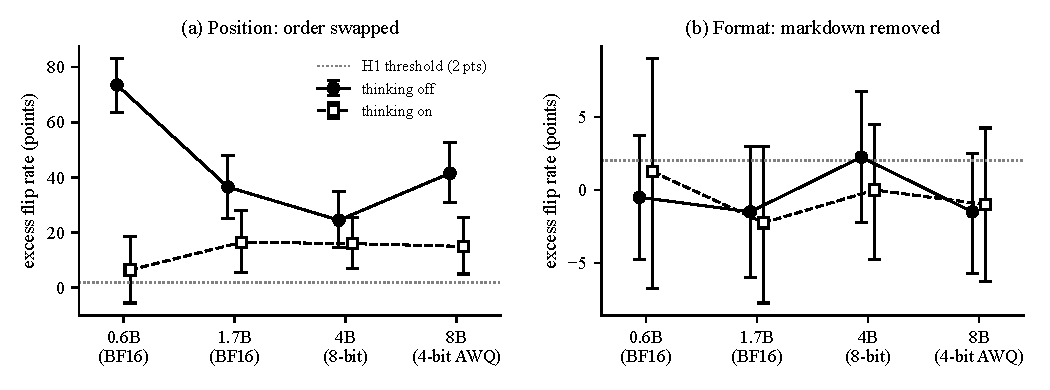
\includegraphics[width=0.97\linewidth]{fig_excess.pdf}
\caption{Excess flip rate per judge setup, with 95\% CIs. Filled circles: thinking off; open squares: thinking
on. Dotted line: the 2-point bar for ``real bias''. (a) Swapping order flips verdicts far beyond noise. (b)
Removing markdown does not, on this measure (see Figure~\ref{fig:pref}b).}
\label{fig:excess}
\end{figure}

\begin{figure}[H]
\centering
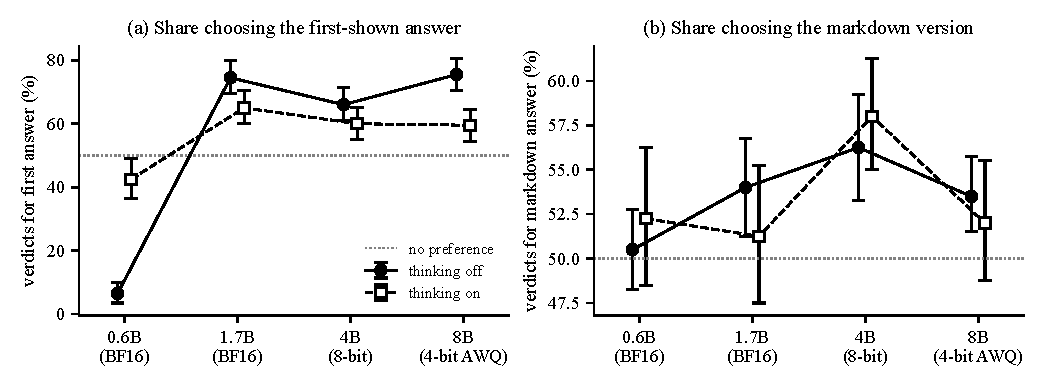
\includegraphics[width=0.97\linewidth]{fig_preference.pdf}
\caption{Which way the judges lean. (a) Share of verdicts for the first-shown answer: 0.6B prefers the
\emph{second} answer, and larger judges prefer the \emph{first}. (b) Share of verdicts for the version that kept
its markdown: slightly above 50\% for mid-size and large judges.}
\label{fig:pref}
\end{figure}

\section{Format results in detail}
\begin{table}[H]
\centering\small
\caption{Format measures. The format excess flip rate stays near 0 because two effects cancel. Removing the
winner's markdown tends to flip the verdict, while removing the loser's markdown tends to keep it (last two
columns). That is why markdown preference is the better measure of format bias.}
\begin{tabular}{l rr rr}
\toprule
Judge setup & Format flip & Format excess flip & Flip when winner stripped & Flip when loser stripped \\
\midrule
0.6B, thinking off & 13.0 & $-0.5$ [$-4.8$, 3.8] & 13.5 & 12.5 \\
0.6B, thinking on & 37.8 & 1.2 [$-6.8$, 9.0] & 40.0 & 35.5 \\
1.7B, thinking off & 15.0 & $-1.5$ [$-6.0$, 3.0] & 19.0 & 11.0 \\
1.7B, thinking on & 19.2 & $-2.2$ [$-7.8$, 3.0] & 20.5 & 18.0 \\
4B (8-bit), thinking off & 15.8 & 2.2 [$-2.2$, 6.8] & 22.0 & 9.5 \\
4B (8-bit), thinking on & 14.0 & 0.0 [$-4.8$, 4.5] & 22.0 & 6.0 \\
8B (4-bit), thinking off & 8.0 & $-1.5$ [$-5.8$, 2.5] & 11.5 & 4.5 \\
8B (4-bit), thinking on & 13.0 & $-1.0$ [$-6.2$, 4.2] & 15.0 & 11.0 \\
\bottomrule
\end{tabular}
\end{table}

\section{Effect of thinking and model size}
\begin{table}[H]
\centering\small
\caption{Change in position excess flip rate when thinking is turned on (paired bootstrap over pairs).}
\begin{tabular}{lrl}
\toprule
Model & Change (points) & 95\% CI \\
\midrule
0.6B & $-67.0$ & [$-82.0$, $-51.5$] \\
1.7B & $-20.0$ & [$-34.0$, $-6.0$] \\
4B (8-bit) & $-8.5$ & [$-19.5$, $+2.5$] (not significant) \\
8B (4-bit) & $-26.5$ & [$-39.5$, $-13.5$] \\
\bottomrule
\end{tabular}
\end{table}
\textbf{Statistical model (proposal's H2).} We fit a GEE logistic regression on flip indicators,
$\text{flip} \sim \text{edit} \times (\log_2\text{size} + \text{thinking})$, clustered by pair. Here
\emph{edit} $=1$ for an order swap and $0$ for a repeat of the same input, so the edit$\times$size and
edit$\times$thinking terms measure how the \emph{excess} flip rate changes. Holm correction covers these two
terms.
\begin{itemize}
\item \textbf{Thinking:} $\beta=-1.55$ (SE 0.17), $p<0.001$. The average effect is \textbf{$-30.5$ points} (CI
$-37.0$ to $-24.5$); excluding 0.6B it is $-18.3$ points ($p<0.001$).
\item \textbf{Model size:} $\beta=-0.06$ (SE 0.08), $p=0.47$. The average effect is $-3.6$ points per doubling (CI
$-6.3$ to $-0.2$). This is inconclusive: the trend is not steady (thinking off: 73.5, 36.5, 24.5, 41.5), and size
is mixed up with 8-bit and 4-bit precision. \textbf{Do not write ``larger models are significantly less
biased.''} The coefficient is not significant, and the CI includes changes both smaller and larger than the
proposal's 3-point smallest effect of interest, so neither an effect nor its absence is established.
\end{itemize}

\section{Agreement with human voters}
\begin{table}[H]
\centering\small
\caption{Agreement with the Arena voter's choice. Accuracy uses the original order (Wilson 95\% CI);
swap-and-average gives half credit when the verdict flips with order. The setups cannot be ranked against each
other at $n=100$.}
\begin{tabular}{lrcrr}
\toprule
Judge setup & Accuracy & 95\% CI & Cohen's $\kappa$ & Swap-and-average \\
\midrule
0.6B, thinking off & 58 & [48, 67] & 0.08 & 50.5 \\
0.6B, thinking on & 61 & [51, 70] & 0.20 & 57.5 \\
1.7B, thinking off & 59 & [49, 68] & 0.22 & 58.5 \\
1.7B, thinking on & 51 & [41, 61] & 0.04 & 56.0 \\
4B (8-bit), thinking off & 60 & [50, 69] & 0.22 & 61.0 \\
4B (8-bit), thinking on & 64 & [54, 73] & 0.30 & 64.0 \\
8B (4-bit), thinking off & 62 & [52, 71] & 0.28 & 62.5 \\
8B (4-bit), thinking on & 66 & [56, 75] & 0.34 & 62.5 \\
\midrule
Baseline: random verdicts (one draw) & 58 & & 0.18 & \\
Baseline: longer answer wins & 57 & & 0.14 & \\
\bottomrule
\end{tabular}
\end{table}
Baselines on the full pools (\texttt{reports/baselines.csv}): longer-answer-wins reaches 57.9\% on the
1{,}000-pair position pool, 57.3\% on the format pool, and 68.8\% ($\kappa=0.38$) on 1{,}284 MT-Bench expert votes.

\textbf{Context for the report:} across all eligible Arena pairs where only one answer used markdown, human
voters picked the markdown answer 56.9\% (2023) and 56.3\% (2025) of the time. This holds after controlling for
length (odds ratio 1.21 / 1.15, $p\le0.009$), so humans are format-biased too.


\section{Run statistics}
\begin{table}[H]
\centering\small
\caption{Per setup: 1{,}000 calls each, 0 invalid answers and 0 retries. ``Truncated'' = thinking runs that hit the
2{,}048-token limit and were closed early (the proposal asks to report this).}
\begin{tabular}{lrrr}
\toprule
Judge setup & Truncated & Mean output tokens & Mean thinking tokens \\
\midrule
0.6B, thinking off & -- & 105 & -- \\
0.6B, thinking on & 6 & 440 & 366 \\
1.7B, thinking off & -- & 175 & -- \\
1.7B, thinking on & 12 & 567 & 477 \\
4B (8-bit), thinking off & -- & 220 & -- \\
4B (8-bit), thinking on & 9 & 612 & 566 \\
8B (4-bit), thinking off & -- & 203 & -- \\
8B (4-bit), thinking on & 7 & 624 & 592 \\
\bottomrule
\end{tabular}
\end{table}

\section{Position bias by data source}
\label{sec:source}
\begin{table}[H]
\centering\small
\caption{Position excess flip by Arena release (the proposal asks for results by source). 2023 has only 16 pairs,
so its CIs are very wide.}
\begin{tabular}{lll}
\toprule
Judge setup & 2023 ($n=16$) & 2025 ($n=84$) \\
\midrule
0.6B, thinking off & 75.0 [53.1, 90.6] & 73.2 [61.3, 83.3] \\
0.6B, thinking on & 21.9 [$-3.1$, 46.9] & 3.6 [$-10.1$, 17.3] \\
1.7B, thinking off & 6.2 [$-21.9$, 34.4] & 42.3 [29.8, 54.2] \\
1.7B, thinking on & 3.1 [$-9.4$, 15.6] & 19.0 [6.0, 32.1] \\
4B (8-bit), thinking off & 9.4 [$-6.2$, 28.1] & 27.4 [15.5, 39.3] \\
4B (8-bit), thinking on & 3.1 [0.0, 9.4] & 18.5 [7.7, 29.2] \\
8B (4-bit), thinking off & 6.2 [$-9.4$, 25.0] & 48.2 [36.3, 60.1] \\
8B (4-bit), thinking on & 9.4 [0.0, 25.0] & 16.1 [4.2, 28.0] \\
\bottomrule
\end{tabular}
\end{table}

\section{Example}
\textbf{Question:} ``Create a sarcastic, meta-style one-liner to promote Deadpool.'' The human voter preferred
answer A (DeepSeek-R1) over B (DeepSeek-V3). The 1.7B judge with thinking off replied [[A]] (``first answer
wins'') in all 10 calls:
\begin{table}[H]
\centering\small
\begin{tabular}{llll}
\toprule
Shown first & Shown second & Judge said & Winner \\
\midrule
A (markdown) & B (markdown) & [[A]] & A \\
B (markdown) & A (markdown) & [[A]] & \textbf{B} \\
A (plain) & B (markdown) & [[A]] & A \\
B (plain) & A (plain) & [[A]] & \textbf{B} \\
\bottomrule
\end{tabular}
\end{table}
The judge picked whichever answer came first. Order decided the verdict, not content.

\section{Data pipeline numbers}
\begin{table}[H]
\centering\small
\begin{tabular}{lrr}
\toprule
Step & 2023 Arena & 2025 Arena \\
\midrule
Loaded & 33{,}000 & 135{,}634 \\
English & 29{,}206 & 71{,}175 \\
Single turn, text only & 25{,}904 & 60{,}895 \\
Clear human winner (no tie) & 18{,}296 & 44{,}299 \\
Length ratio $\le 2$ & 9{,}463 & 25{,}567 \\
No code or tables, deduplicated, fits the prompt & 8{,}325 & 16{,}052 \\
Markdown in both answers, strips cleanly & 169 & 11{,}308 \\
\bottomrule
\end{tabular}
\end{table}
\begin{itemize}
\item \textbf{Frozen pools} (seed 261): a 1{,}000-pair position pool (2023) and a 1{,}000-pair format pool (167
from 2023, 833 from 2025). The 100 midterm pairs come from the format pool.
\item \textbf{Markdown removal check}: 2{,}400 of 2{,}400 stripped answers keep the exact same words. These
are the 1{,}200 pairs of the format pool plus its reserve at freeze time (file
\texttt{reports/strip\_validation.csv}). A further 160 candidate answers failed the check and were excluded
before freezing.
\item \textbf{Audit} of 50 pairs (first pass by an AI reviewer, file \texttt{reports/manual\_audit.csv}; team
sign-off pending). Meaning and wording were kept in 100 of 100 answers. Two answers lost readable list structure
(three-level nested bullets). Their pairs were swapped out of the frozen format pool for reserve pairs, but they
are still in the 100-pair midterm set, which was drawn earlier. Removing them changes results by at most 1.3
points.
\end{itemize}


\section{Progress against the proposal}
\begin{table}[H]
\centering\small
\begin{tabularx}{\linewidth}{>{\raggedright\arraybackslash}p{4.6cm} >{\raggedright\arraybackslash}p{2.3cm} X}
\toprule
Proposal item (week) & Status & Notes \\
\midrule
Data check, frozen pools (W5) & Done & 1{,}000-pair position and format pools, seed 261, hashes recorded. \\
Pilot (W5) & Done locally & Planned with 0.6B and 8B thinking; run instead with 0.6B and 1.7B (520 calls), then this 8{,}000-call run. No hosted-API pilot yet. \\
Frozen evaluation contract (W5) & Done & \texttt{docs/evaluation\_contract.md}: prompt, settings, metrics, analysis rules. \\
Harness + estimates on two sizes (W7) & Done, ahead & All four sizes, both modes. \\
Compute: Kaggle T4, vLLM, FP16 & Changed & No Kaggle. Mac (MLX) for 0.6B--4B; RTX 3070 (vLLM) for 8B. 4B 8-bit, 8B 4-bit. OpenRouter and Together do not serve these models (\texttt{docs/api\_comparison.md}). \\
Sample size & Partial & 100 of 1{,}000 pairs per pool. \\
Sampling-mode check & Not run & Thinking off with thinking settings; planned for 200 pairs per size. \\
Paraphrased-prompt check & Not run & Prompt is written (\texttt{src/dsc261/judge.py}). \\
Full pre-registered regression & Partial & Done here for position only. Format terms, size$\times$thinking, Holm over \{position, format\}$\times$\{size, thinking\} and the $\pm$3-point equivalence tests are still to do. \\
Audit sign-off; official 2023 file & Pending & Each member confirms their 10 audit pairs; re-run notebook 01 with an HF token. \\
Human agreement on MT-Bench & Data ready & 1{,}284 turn-1 expert votes prepared, not yet judged. \\
H3 best-of-$n$ (UltraFeedback) & Data ready & 500 prompts $\times$ 4 answers with gold scores and brackets built, not yet judged. \\
Full study, H1--H3 (W9--10) & Not started & Manifest of 151{,}296 calls ready (16{,}912 per setup vs the proposal's $\sim$13K, because the position and format pools are separate). Estimated about 20 GPU-hours on an L4 (about \$16, assumed throughput) or about \$87 on Featherless (\texttt{api/cost\_projection.csv}). \\
\bottomrule
\end{tabularx}
\end{table}
\textbf{Next steps (suggested):}
\begin{enumerate}
\item Run the full 1{,}000-pair pools for all four sizes at full precision on one GPU backend.
\item Run the sampling-mode and paraphrased-prompt checks.
\item Run H3 and MT-Bench agreement.
\item Fit the full pre-registered regression (position and format, size $\times$ thinking, equivalence tests).
\item Team sign-off of the audit; re-run on the official 2023 Arena file.
\end{enumerate}

\section{Caveats to mention in the report}
\begin{itemize}
\item \textbf{Sample size}: 100 of the planned 1{,}000 pairs, so the intervals are wide. These are interim results.
\item \textbf{Multiple comparisons}: the per-setup CIs are not adjusted. With a Bonferroni adjustment over 8 setups,
5 position effects still have a lower bound above 2 points: 0.6B off [58.5, 86.0], 1.7B off [20.0, 52.9], 4B off
[10.5, 38.5], 4B on [4.0, 29.0] and 8B off [26.0, 56.0]. 1.7B on and 8B on both drop to [1.0, \ldots].
\item \textbf{Precision}: 4B is 8-bit and 8B is 4-bit because of hardware limits (the plan said full precision).
Size comparisons therefore mix size with compression.
\item \textbf{Sampling settings}: thinking on and off use different sampling settings, as in the model card. The
check that separates the two (thinking off with thinking settings) has not been run yet.
\item \textbf{0.6B with thinking} looks unbiased (6.5 points) only because it is very noisy (36.5\% of repeats
disagree). It still leans toward the second answer (42.5\% first-slot).
\item \textbf{Subset}: the 100 pairs are markdown-heavy and 84\% from 2025. For 6 of the 8 setups, position bias
is larger on the 2025 pairs. The exception is 0.6B, which is strongly biased on both (Section~\ref{sec:source}).
Only 16 pairs come from 2023, so the 2023 numbers are very uncertain.
\item \textbf{Format edit}: only headings, bold and bullets are removed; italics and numbered lists stay.
\item \textbf{Data source}: the 2023 Arena file came from a public mirror (the official one needs a login). Licences:
2025 Arena CC-BY-4.0; MT-Bench CC-BY-4.0; UltraFeedback MIT (\texttt{docs/dataset\_records.md}).
\item \textbf{Robustness}: removing the 2 audit-flagged pairs changes results by at most 1.3 points. Repeated runs
produced different outputs, except 1.7B with thinking off, where 21 of 200 repeats were word-for-word identical
(a near-deterministic model, not a seed error). There were 0 invalid answers anywhere.
\item \textbf{Backends}: 0.6B--4B ran on MLX (Mac) and 8B on vLLM (GPU); the proposal planned vLLM for all.
\end{itemize}


\section{For the report writers}
\begin{itemize}
\item \textbf{References}: reuse the proposal's references [1]--[11]. Also cite UltraFeedback (Cui et al., ICML
2024), the Qwen3 technical report/model card (sampling settings) and AWQ (Lin et al., MLSys 2024) for the 8B model.
\item \textbf{AI usage disclosure} (suggested): ``We used Claude to help write the data pipeline, judge harness and
analysis code, to run the first pass of the stripping audit, and to draft text. All numbers come from released
scripts; the team verified the claims.''
\item \textbf{Team contributions}: map names onto the proposal's roles: Member 1 harness and logging, 2 stripping
and audits, 3 data pools and human agreement, 4 UltraFeedback bracket, 5 statistics, figures and contract.
\item \textbf{Safe one-line claims}: ``Order swaps change verdicts 15--73.5 points beyond noise in 7 of 8 setups'';
``Thinking lowers this by 18--30 points but does not remove it''; ``Markdown removal rarely flips verdicts, but four
setups prefer the markdown version 53.5--58\% of the time''.
\item \textbf{Avoid}: ``larger models are less biased'' (not established); ``0.6B with thinking is unbiased'' (it is
noisy); ``8B is the most accurate judge'' (agreement CIs overlap).
\end{itemize}

\section{Files}
\begin{tabularx}{\linewidth}{>{\ttfamily\raggedright\arraybackslash}p{6.3cm} X}
\toprule
\normalfont\bfseries File & \textbf{What it is} \\
\midrule
report/results.csv & all numbers in Table~\ref{tab:main} (and more columns) \\
report/runs.csv & calls, invalid answers, truncation, token counts per setup \\
report/stats.json, extra.json & statistical model, baselines, robustness numbers \\
report/fig\_excess.pdf, fig\_preference.pdf & the two figures (vector, ready to paste) \\
notebooks/06\_midterm\_results.ipynb & analysis notebook \\
data/processed/pilot\_pairs.parquet & the 100 pairs \\
api/pilot\_local/, api/midterm\_remote/ & raw judge logs (every call and its full output) \\
docs/evaluation\_contract.md & frozen rules: prompt, settings, metrics \\
\bottomrule
\end{tabularx}
\end{document}
